\documentclass{article}

\usepackage{graphicx}
\graphicspath{ {./images/} }
\usepackage{textcomp}
\usepackage[T1]{fontenc}
\usepackage{fancyhdr}
\usepackage{hyperref} % Hyperlinks

\pagestyle{fancy}
\fancyhf{}
\rhead{Magic feet}
\lhead{Krzysztof Dąbrowski, Marharyta Kruk}
\rfoot{Page \thepage}

\title{Final project for Python programming and Data visualization course}
\author{Marharyta Kruk, Krzysztof Dąbrowski}
\date{\today}

\begin{document}

\maketitle
\tableofcontents
\newpage

\section{Intro}
Our task was to make web based application written in Python. Out application presents a graphical visualization of a device for monitoring walk habits and patterns of elderly and disabled persons.
\newline
This device provides real-time measurements of pressure of feet on the ground, so our application's components are real-time based.
\subsection{How to run}
Before starting project make sure to connect to PW VPN to allow access to data API.

Project is containerized with Docker. To start it simply run \texttt{docker-compose up} in main directory. After that step open \href{http://localhost:8050}{localhost:8050} in browser.

\section{Technical details}
\subsection{General}
We use \textit{Plotly Dash} libraries for our project. We have chosen them because of their elegant simplicity and wide functionality. All elements in our project are parts of the Dash layout, each element represents dash core or html components. We also use \textit{dash core Store components} to store some data(Current person id and data about last anomaly), so this data is stored in secure way. We store current person id in Session store, so each user can have their own page which will not affect the others.
\subsection{Persons}
We have access to the data of 6 persons, so we've implemented tabs that changes current person information. As was mentioned above, we store this information in session storage, co current person can be different for different sessions. Current person id manages all other components. We have implemented tabs via \textit{dash core components Tabs}.
\subsection{Storage}
For data storage we have chosen to use \textit{Redis} database, because of its simplicity. Data acquisition starts along with the \texttt{api\_cache} module. In our index program we have variable \textit{store}, which is an instance of Redis database, connected with our running database. Next, we use data from Redis storage for real-time visualization. For visualizations, we use only 20 last records, because it is an optimal amount for fast real-time visualizations. Caching module stores last 10 minutes of data.
\subsection{Structure and components}
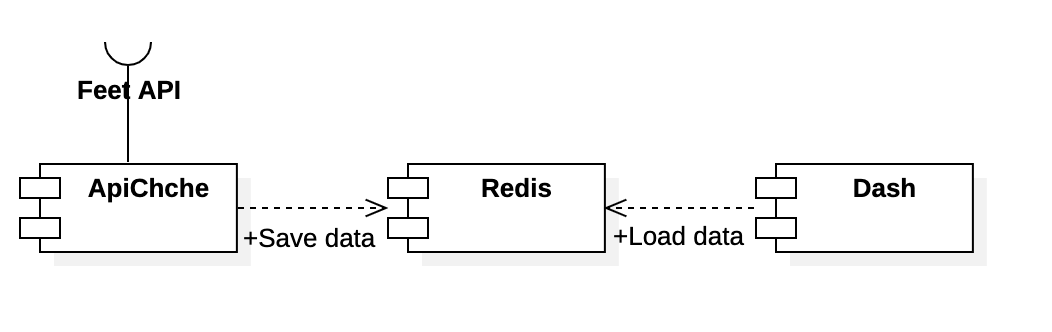
\includegraphics[width=12cm]{MagicFeetComponents}
\newline
All our components update every second, catching new information. We use functions with update\_ prefix to draw our figures. These components have elements in layout as Putput and time with
current person id as Input. We use time(interval\_component) for updating with time. Some figures have more Outputs and Inputs.

\texttt{Update\_anomal\_histogram} function handle our anomaly histogram. It has 2 Outputs, one of which is layout component and another is hidden storage for information about last anomaly, and a State. We use State because we can't have 2 components with same Output and we can't have same Input and Output in one component. For this function we use State for checking current information about last anomaly(because we can't use it as Input when we already have it as Output)

Component \texttt{Update\_single\_sensor\_indicator} use 3 Inputs: time, current person id and current sensor tab, so w can switch between sensors.

We also have label with information about last anomaly. It is tricky; we show this label only if we have some information. \texttt{Update\_last\_anomaly} waits for changing value of last\_anomaly store with a help of modified-timestamp value.
\newline
We have a bunch of functions with \texttt{make\_} prefix. When update\_ functions manage our layout and collect data, make\_ functions create figures. It was possible to unite them, but we separate them, because we want to make our code more clear and readable.
\newline
All our project we have packed in Docker container, so it is easy to build it and run.
\section{Visual design}
All our components we have chosen to show variation of our data, so each figure provides quantitative information.
\newline
We use table for general picture of our data. Our table represent Dash core component Graph, which uses component Table from Plotly graph objects. This decision was made because we use dictionaries for building table, and we also store data in Redis database in the form of dictionary. Another plus of using this table is possibility to colour cells depending on their values (as we have implemented).
\newline
Feet animation is using for visualization of pressure which is made from sensor's values
\newline
We use Indicator for clear demonstration how values on the sensors change and what is the difference between previous and current value. We use here the same tabs, co user can easily switch between sensors.
\newline
For anomalies we use histogram of anomalies, which we have chosen because it is good tools for visualization how huge is number of anomalies and how it changes with time. We also have label with information about last anomaly, so when histogram is empty, we can learn when was last anomaly and on which sensor.
\newline
So, for good appearance we use some our custom css styles, which are placed in \textit{asserts} folder. We style our page with thoughts about simplicity, accuracy and intuitiveness of interaction with our components.

\end{document}